
%
%  $Description: Author guidelines and sample document in LaTeX 2.09$
%
%  $Author: ienne, modified by Laurent George $
%  $Date: 2012/02/02 15:20:59 $
%  $Revision: 1.5 $


\documentclass[times, 10pt,twocolumn, a4paper]{article}
\usepackage{latex8}
\usepackage{epsfig, hhline}
\usepackage{amssymb}
\usepackage{vmargin,array,multirow,float,shadow,times, euscript}
\usepackage{amsmath}
\usepackage{algorithmic}
\usepackage[ruled,vlined]{algorithm2e}
\usepackage{pdftricks}
\usepackage{stmaryrd}


\newtheorem{property}{Property}
\newtheorem{assumption}{Assumption}
\newtheorem{theorem}{Theorem}
\newtheorem{definition}{Definition}
\newtheorem{lemma}{Lemma}
\newtheorem{remark}{Remark}
\newtheorem{constraint}{Constraint}
\newtheorem{corollary}{Corollary}
\newtheorem{condition}{Condition}

\def\QED{\mbox{\rule[0pt]{1.5ex}{1.5ex}}}
\def\proof{\noindent{{\textbf{Proof}: }}}
\def\endproof{\hspace*{\fill}~\QED\par\endtrivlist\unskip \vspace{1\baselineskip}}

\newcommand{\dbf}[1]{\operatorname{dbf}(#1)}

\algsetup{
	indent=2em,
	linenosize=\small,
	linenodelimiter=\
}

%\newenvironment{accolade}{\begin{centering} $$ \left\{ \begin{array}{l}}{\end{array} \right. $$ \end{centering}}


%-------------------------------------------------------------------------
% take the % away on next line to produce the final camera-ready version
\pagestyle{empty}

%-------------------------------------------------------------------------
\begin{document}

\title{Describing the C-Space of Asynchronous Periodic Task Systems using
Definitive Idle Times}

\author{Thomas Chapeaux, Paul Rodriguez\\
Universit\'e Libre de Bruxelles\\ tchapeau@ulb.ac.be, paurodri@ulb.ac.be \\
% For a paper whose authors are all at the same institution,
% omit the following lines up until the closing ``}''.
% Additional authors and addresses can be added with ``\and'',
% just like the second author.
\and
Laurent George\\
ECE Paris\\
First line of institution2 address\\ Second line of institution2 address\\
lgeorge@ece.fr\\
}

\maketitle
\thispagestyle{empty}

\begin{abstract}
	Lorem ipsum dolor sit amet, consectetur adipiscing elit. Nulla lobortis mi vel
turpis ultricies vulputate vel at arcu. Curabitur lectus metus, rutrum sed malesuada ut, mollis sit amet mauris. Integer dapibus in risus et porttitor. In hac habitasse platea dictumst. Maecenas dolor libero, suscipit porta consequat eu, consequat non orci. Sed tortor neque, tincidunt congue cursus sit amet, luctus id ipsum. Aenean tempor est nisl, at dictum metus elementum iaculis.\\

Keywords: Real-time systems, C-space, WCET, sensitivity analysis
\end{abstract}



\section{Introduction}

	Abstract models for real-time systems often require the determination of the
	(worst-case) computation time of a job (WCET), a value highly dependent on the
	platform on which the application will be deployed.\\

	The \emph{C-space} of a real-time system is, intuitively,
	the set of WCET values for which this system would be feasible. A
	precise and efficient description of its C-space would allow to quickly decide
	if a system is feasible on a given platform.\\

	In this section the current description of the C-space of synchronous
	constrained systems, which has been mostly covered by \cite{george2009characterization}, is reviewed.

	\subsection{Model}

		We consider a discrete timeline and tasks systems $\tau$ comprised of periodic concrete
		tasks with constrained deadlines on uniprocessor platforms. Each task
		$\tau_i$ is represented by a tuple $(O_i, C_i, D_i, T_i)$ where $O_i$ is the offset value,
		$C_i$ the WCET, $D_i$ the relative deadline and $T_i$ the period.
		The constrained deadline property implies that $D_i \leq T_i \; \forall i$. In
		the following, we differentiate between \emph{synchronous systems} (where $O_i
		= 0 \; \forall i$) and \emph{asynchronous systems} (which are not synchronous).\\

		For those systems, the \emph{Earliest Deadline First} (EDF) algorithm, in
		which jobs are prioritized according to their absolute deadline, has been
		shown to be optimal \cite{liu1973scheduling}, which means it
		correctly schedules any feasible system within that group.\\

		Furthermore, the following notations are used:
		\begin{itemize}
			\item $\tau = \{\tau_0, \cdots, \tau_{n-1}\}$
			\item $H = \operatorname{lcm}(T_0, \cdots, T_{n-1})$
			\item $O_{max} = \max (O_0, \cdots, O_{n-1})$
			\item An \emph{idle time} is an instant $t$ at which each job that arrived
			\emph{strictly} before $t$ has finished its execution.
			\item A \emph{busy period} is a time interval during which there is always
			at least one unfinished job available in the system and maximal
			with this property. Any busy period starts and ends
			with an idle time.
			\item The interval between the initial time and the first
			idle time is called the \emph{first busy period}.
		\end{itemize}

	\subsection{The DBF feasibility test}

	We recall the necessary and sufficient condition explained in \cite{baruah1999generalized, baruah1990algorithms}, based on the demand-bound function.

	\begin{definition}
		The \textbf{demand-bound function (DBF)}
		defined for a task set $\tau$ and noted $\dbf{t_1, t_2}$, is equal to
		the maximal cumulated execution time of jobs of $\tau$ contained in the
		closed interval $[t_1, t_2]$.
	\end{definition}

	Mathematically,
	\[
		\dbf{t_1, t_2} = \sum_{i=0}^{n-1} n_i(t_1, t_2) \, C_i
	\]
	where $n_i(t_1, t_2)$ is the number of jobs of task $i$ which arrival times
	and deadlines are both in the closed interval $[t_1, t_2]$.\\

	The values of the $n_i$ are given by
	\[
		n_i(t_1, t_2) =
		\left\llbracket
			\left\lfloor
				\frac{t_2 - O_i - D_i}{T_i}
			\right\rfloor -
			\left\lceil
				\frac{t_1 - O_i}{T_i}
			\right\rceil + 1
		\right\rrbracket_0
	\]
	where $\llbracket x \rrbracket_0$ stands for $\max \{ 0, x \}$.\\

	A necessary and sufficient condition of feasibility can easily be written
	based on the DBF:

	\begin{theorem}
	\[
		\begin{array}{c}
			\{\tau_1, ..., \tau_n\} \: \text{is feasible}  \iff \\
			\dbf{t_1, t_2} \leq t_2 - t_1 \; \forall \: 0 \leq t_1 \leq t_2
		\end{array}
	\]
	\end{theorem}

	\subsection{C-space of synchronous systems}

		\subsubsection{Definition}

			The authors of \cite{george2009characterization} give the following definition of the C-space:
			\begin{definition}
				The \textbf{C-space} of a task system $\tau$ is a region of $n$ dimensions (where each dimension denotes the possible $C_i$ of a task of $\tau$) such that for any vector $C = \{ C_0, \cdots, C_{n-1}\}$ in it, $\tau$ is feasible.
			\end{definition}

%Thus, with a good description of the C-space, it is easy to check if a given vector of $C_i$ value (given e.g. when deploying the application on a specific platform) allows the system to be scheduled or not.

		\subsubsection{Description using DBF}
			\label{sct:cspaceDescr}

			As explained in \cite{nemhauser1988integer}, a region of $\mathbb{N}_0^n$ such as the C-space can be described by a \emph{polytope}, or a list of parametric linear constraints (called the \emph{formulation}). The constraints must be conditions which can unequivocally decide if a point is included in the region or not. In the sequel we give a formulation for the C-space in $\mathbb{N}_0^n$ (For a formulation in $\mathbb{N}^n$, we can add $C_i \geqslant 1 \; \forall i$ in the list of constraints).\\

			The DBF test gives us a list of inequations on the WCET values of the task set which together are a necessary and sufficient condition of feasibility. They can all be written in the following way:
			\[
				\sum_{i=0}^{n-1} n_i(t_1, t_2) \, C_i \leq t_2 - t_1 \; \forall \: 0 \leq t_1 \leq t_2
			\]
			Note that for a given $t$, we have that the $n_i(t)$ are
			constant (w.r.t. the $C_i$). Those inequations are thus indeed linear.\\

			However, this description contains an infinite number of constraints, most of
			which are redundant. While this does not harm the precision of the
			test, the smallest description is preferred as it can greatly
			reduce the computation time of practical feasibility tests using this system
			of inequations. In Section~\ref{sct:removeRedundancy} a method to reduce the size of this set of constraints is given.

	\subsection{Removing redundancy}
		\label{sct:removeRedundancy}

	In the synchronous case, is has been shown that the inequations corresponding
	to every interval $[0, t]$ (with $t$ a job deadline happening before $H$) are
	necessary and sufficient to test the feasibility of a system.\\

	Even then, the number of inequations to consider is exponential in the number
	of tasks. While it has been shown that constraints that cover intervals ending
	after the end of the first busy period are also redundant, this value depends on the $C_i$ and is
	therefore not usable, or at least not for the purposes of this paper. The
	following concept is thus introduced, which is similar to the end of the busy period but does not depend on the execution times.

	\begin{definition}
		A \textbf{definitive idle time} (DIT) is a time $t$ such that every job
		released strictly before instant $t$ has its absolute deadline before or at instant $t$.
	\end{definition}

	\begin{definition}
		The earliest DIT occurring in the system strictly after $t=0$ is called the
		\textbf{first DIT} and is noted $t_d$.
	\end{definition}

	\begin{remark} (from the definitions):
		\begin{itemize}
			\item Contrary to other idle times, DITs are independent of the
			scheduling or the execution times of the jobs.
			\item In a feasible system, every DIT is an idle time.
			\item In a feasible system, the first DIT happens after the end of the
			first busy period.
			\item As any $kH$ with $k \geqslant 0$ is a DIT in synchronous systems, we have at least $t_d
			\leqslant H$ in this case.
		\end{itemize}
	\end{remark}

	The value of the first DIT can be found by solving the following modular equation system:
	\[
		t_d = \min
		\left( t \; s.t. \; \forall i:
			\left\{
				\begin{array}{c}
					t > 0 \\
					t \equiv a_i \; (mod \; T_i) \\
					a_i \in [D_i, T_i]
				\end{array}
			\right.
		\right)
	\]
	The authors of \cite{george2009characterization} give a method to solve this system for cases in which periods are pairwise coprime.\\

	Every DIT being an idle instant, the execution of the system after a DIT does
	not depend on the execution before it. Because the synchronous arrival pattern is
	the worst case [citation needed], it is sufficient for the DBF test to only
	consider intervals $[0, t]$ with $t$ being a deadline before or at the first DIT.\\

	To summarize, we reduced the description of the C-space from an infinite number
	of constraints to only those where $t_1 = 0$, $t_2 \leqslant t_d$ and
	values of $t_2$ correspond to job deadlines. Note that the number of
	constraints is still exponential in the number of tasks.

	\subsection{Our work}
		In this paper, we extend the work of \cite{george2009characterization} to the
		asynchronous case. In section \ref{sct:asyncDIT}, we present an extension of
		the concept of DIT adapted to the asynchronous case called first periodic DIT
		($t_d$), along with an algorithm to determine its existence and value for any system. In Section
		\ref{sct:asyncCspace}, we show how to describe the C-space of an asynchronous
		system based on the DBF test, and we show why the interval $[t_d, t_d + H]$ is
		sufficient to consider. In section ???, we present a simulation where we find that........

\section{DIT in asynchronous systems}
	\label{sct:asyncDIT}

	\subsection{Definition}

		In an asynchronous system, the first DIT may happen before $O_{max}$, i.e. before all tasks are in the system. We thus introduce the following notion:

		\begin{definition}
			The \textbf{first periodic DIT} (FPDIT) of a system is the earliest DIT occurring
			strictly after $O_{max}$.
		\end{definition}

		By a slight abuse of notation, it will also be noted $t_d$. Note that in the
		synchronous case the first periodic DIT is also the first DIT.

	\subsection{Existence condition}
  \label{sct:FPDITexist}
		As in the synchronous case, the problem of existence of the FPDIT
		can be written as a system of modular equations:
		\[
			\begin{array}{l}
				\exists ? \; t_d \; s.t. \; \forall i \; :\\
				\left\{
					\begin{array}{l}
						t_d > O_i \\
						t_d - O_i \equiv a_i \; (mod \; T_i) \\
						a_i \in [D_i, T_i]
					\end{array}
				\right.
			\end{array}
		\]

		This system is guaranteed to have at least one solution modulo $H$ for given
		values of $a_i$ if the following condition is respected:
		\[
			a_i + O_i \equiv a_j + O_j \; (\operatorname{mod} \; \operatorname{gcd}(T_i,
			T_j)) \; \forall i,j
		\]
		which means that there could be systems with no FPDIT.
		We now present an example of such a system.\\

		\begin{center}
		\begin{tabular}{|r|c|c|c|c|}
		 \hline
		  & $O_i$ & $C_i$ & $D_i$ & $T_i$ \\
		 \hline
		 $\tau_1$ & 0 & $C_1$ & 3 & 4\\
		 \hline
		 $\tau_2$ & 2 & $C_2$ & 7 & 8\\
		 \hline
		\end{tabular}
		\end{center}
		~\\

		Here, the possible values of $a_1$ are 3 and 4, and the possible values
		of $a_2$ are 7 and 8. For a FPDIT to exist, one of the following
		conditions must be fulfilled:
		\[
		\left[
		\begin{array}{c}
			3 + 0 \equiv 7 + 2 \; (\operatorname{mod} \; 4 ) \\
			3 + 0 \equiv 8 + 2 \; (\operatorname{mod} \; 4 ) \\
			4 + 0 \equiv 7 + 2 \; (\operatorname{mod} \; 4 ) \\
			4 + 0 \equiv 8 + 2 \; (\operatorname{mod} \; 4 ) \\
		\end{array}
		\right.
		\]
		However those four conditions cannot be satisfied, which means the system has
		no FPDIT (and no other DIT than $t=0$).

	\subsection{Solving the modular system}
		Finding the FPDIT of a system is similar to finding a synchronous instant of
		this system (an instant at which all tasks release a job simultaneously), but
		with weaker constraints. That is, the FPDIT is an instant after the last
		deadline of all tasks, but before the next arrival time of all tasks. Finding
		a synchronous instant is equivalent to finding a solution $t$ for the
		following set of constraints :
		\[
			\left\{
			\begin{array}{l}
				t \geqslant O_i \: \forall \: \tau_i \in \tau \\
				t \equiv O_i \; (mod \; T_i) \: \forall \: \tau_i \in \tau \\
			\end{array}
			\right.
		\]
		which is very similar to an instance of the Chinese Remainder Problem (CRP). It
		is not possible to directly use a solver for the CRP (such as Gauss's
		algorithm \cite{gauss1965disquisitiones}) as in a task system, $T_i$ values could have common factors.
		However, the instance can be modified (each constraint with a non-prime period can be split into powers of primes
		without changing the solution if there is one) in order to make the problem
		solvable through applying a solution for the CRP. \\

		Now that we have a solver for the problem of finding a synchronous instant, we
		actually also have a solver for finding the FPDIT. The problem of finding the
		first DIT is the same as finding all the possible DIT then taking the minimum.
		Each of those DIT corresponds to a unique combination of $a_i$ values (one
		for each task). Finding one of such DIT is the same problem as finding a
		synchronous instant :
		\[
			\left\{
			\begin{array}{l}
				t \geqslant O_i + a_i \: \forall \: \tau_i \in \tau \\
				t \equiv O_i \; (mod \; T_i) \: \forall \: \tau_i \in \tau \\
			\end{array}
			\right.
		\]
		all DITs can be found by solving the equivalent CRP problem for all
		combinations of $a_i$ values. This is however very inefficient as there are
		exponentially many different combinations of $a_i$ values in the number of
		tasks.\\

		A better method for finding the FPDIT consists in splitting Gauss's algorithm
		into two separate parts. The global structure is simply a sum of factors, each
		term being dependent on which $a_i$ value is chosen. A major speedup can
		be achieved by first computing all possible terms for each task (only one
		modular inverse must be computed per task that way) then creating all possible DIT values
		by summing the terms in all possible ways. The number of results is still
		exponential in the number of tasks, but the only operation that is repeated
		exponentially many times is now a sum.

	\subsection{Simulation}

	We wanted to quantify how much systems have a FPDIT........

	We generated task systems by
	\begin{itemize}
		\item Generating utilization values with the \texttt{UUniFast} algorithm described in \cite{bini2005measuring}, with parameters
		\begin{itemize}
			\item $U_{tot}$ (system utilization) chosen uniformly between 0.25 and 0.75
			\item $n$ (number of tasks) equal to 3
		\end{itemize}
		\item Choosing the $T_i$ uniformly between 5 and 20, which also gives us the $C_i = \lfloor U_i \, T_i \rfloor$
		\item Choosing the $O_i$ with a normal distribution of mean $T_{min}$ and standard deviation $\frac{T_{max} - T_{min}}{2}$
		\item Choosing the $D_i$ uniformly in the interval $[T_i - \frac{T_i - C_i}{CDF}, T_i]$, where the $CDF$ is called \emph{Constrained Deadline Factor}.
	\end{itemize}
	and then computed the value of the FPDIT.\\

	We use the CDF because........\\

	\begin{figure}[h]
	\begin{center}
		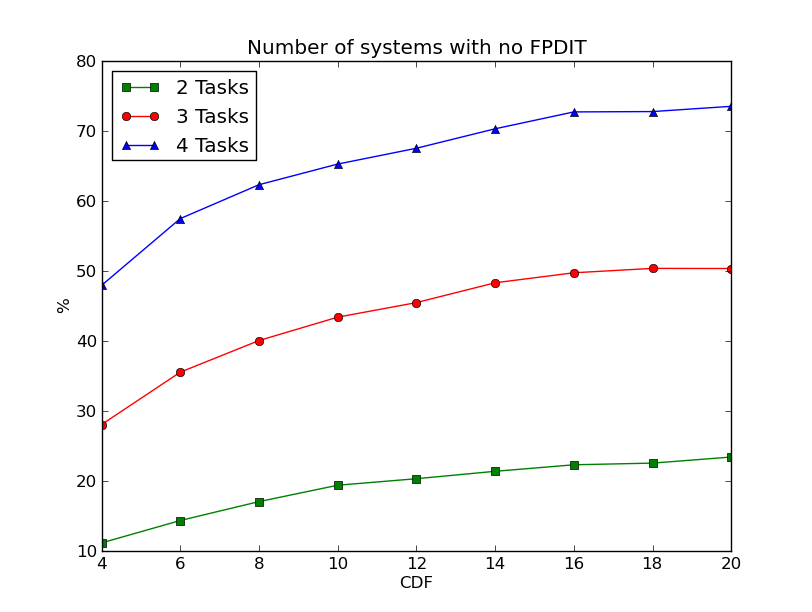
\includegraphics[width=0.5\textwidth]{python-simulation/plots/nofpdit.png}
	\end{center}
	\caption{Evolution of the existence of FPDIT with the CDF}
	\label{fig:noFPDIT}
	\end{figure}

	The result are represented in Fig. \ref{fig:noFPDIT}. We observe that the more we are close to the implicit deadline case, the less systems have FPDIT.

\section{C-space of asynchronous systems}
  \label{sct:asyncCspace}

  \subsection{Description using DBF}

  The description we presented in Section \ref{sct:cspaceDescr} was general, and is thus still relevant. Therefore the C-space is still accurately described by the following infinite number of constraints:$$\sum_{i=0}^{n-1} n_i(t_1, t_2) \, C_i \leq t_2 - t_1 \; \forall \: 0 \leq t_1 \leq t_2$$

  However, the method used in the synchronous case to remove redundancy does not apply here. A more general approach is presented in the following section.

  \subsection{Removing redundancy}

\subsubsection{Job arrival and deadline}

Consider an interval $[t_1, t_2]$. If $t_2$ is an instant without any job deadline, then by definition the value of $\dbf{t_1, t_2}$ will be equal to $\dbf{t_1, t_2^*}$, where $t_2^*$ is the latest deadline before $t_2$.\\

A similar argument can be made if $t_1$ is an instant without any job arrival (and $t_1^*$ is the earliest arrival after $t_1$). We can thus restricts ourselves to intervals where $t_1$ is an instant with at least one job arrival, and $t_2$ is an instant with at least one job deadline.

  \subsubsection{Feasibility interval}

  First let us recall how an asynchronous system behaves under an optimal scheduler, for example EDF.\\

\begin{figure}[h]
	\[
		\begin{array}{r||c|c|c|l}
			& \text{Incomplete} & \text{Transitive} & \text{Stationary} & \cdots \\
			\text{Name} & \text{period} & \text{period} & \text{period}  & \\
			\hline
			\text{size} & O_{max} & H & H & \cdots \\
			\hline
			t \geqslant & 0 & O_{max} & O_{max} + H & \cdots
		\end{array}
	\]
	\begin{center}
	\caption{Behavior of an asynchronous system under EDF.}
	\label{fig:asyncBehavior}
	\end{center}
\end{figure}

As shown in Fig. \ref{fig:asyncBehavior}, the system begins in the \emph{incomplete period}, where all tasks are not in the system. Then, after $O_{max}$ time units, every tasks is in the system and the \emph{transitive period} begins. Then, after $O_{max} + H$ time units, the system is faced with the same pattern of arrival as in $O_{max}$. However, because in $O_{max} + H$ every task is in the system and in $O_{max}$ some were missing, the state of the system will be different. The \emph{stationary period} then begins. It is only after $O_{max} + 2H$ time units that the system comes back into a state in which we can be sure it has been before.\\

For this reason, as explained in \cite{leung1982complexity}, it is sufficient to check for intervals included in the interval $[O_{max}, O_{max} + 2H]$, which has an exponential length in the number of tasks.

\subsubsection{Using the first periodic DIT}

The FPDIT, if it exists, must occur in the transitive period. Indeed, it cannot occur in the incomplete period by definition ($t_d > O_{max}$) and if it occurred in the $k^{th}$ stationary period, another DIT should have occurred in the transitive period at instant $t_d - k H$ (a contradiction).\\

As the FPDIT happens when all tasks are in the system, we know that the system will arrive in the exact same state one hyperperiod later ($t_d + H$). We can thus restrict the DBF test to intervals included in the interval $[t_d, t_d + H]$, if the FPDIT exists. This will always be a better interval than $[O_{max}, O_{max} + 2H]$ and if the first periodic DIT does not exist (which can be verified as explained in Section \ref{sct:FPDITexist}), the latter interval can be used.\\

(Remarque : Sans appliquer le simplexe ou un truc comme ça, si un DIT existe on divisera toujours par exactement 4 le nombre de contraintes ??)

\subsubsection{Redundancy as an integer linear problem}

The general problem of redundancy of a new linear constraint $C \, X \leq d$ w.r.t. a set of previous linear constraints $A \, X \leq B$ in an ILP can itself be written as the following ILP:

\begin{figure}[h]
$$z = \max C \, X$$
s.t.
\[
\begin{array}{rccc}
	A & X &\leq & B \\
	C & X &\leq & d + 1
\end{array}
\]
with
\[
	\begin{array}{ccc}
		A & : & [k,n] \text{ matrix}\\
		B & : & [1,n] \text{ matrix}\\
		C & : & [n,1] \text{ matrix}\\
		X & : & [1,n] \text{ matrix}\\
		d & : & \text{integer}
	\end{array}
\]
\caption{Redundancy of $CX \leq d$ w.r.t. $A X \leq B$ as an ILP}
\end{figure}

Indeed, if the maximization returns $z=d+1$, it means that there are some integer values accessible with the previous constraints that the new constraint forbids. On the other hands, if the maximization returns $z \leq d$, it means that the limitation expressed in the new constraint is already enforced by the previous constraints. Therefore $z \leq d$ is a necessary and sufficient condition of redundancy of the new constraint.\\

Such a linear problem can be solved by the simplex algorithm. However, in our case the problem is not exactly the same as we have a set of constraints and we want to find all redundant constraints within. A naive method would be to test each constraint against all the others. We present a similar method with an efficient preprocessing when most constraints are redundant in Algorithm \ref{alg:prunRedun}.\\

\begin{algorithm}
\caption{Removing redundancy from CSPACE}
\label{alg:prunRedun}
	\begin{algorithmic}[1]
		\STATE $CSPACE$ : set of constraints
		\STATE $S \leftarrow \emptyset$
		\STATE \COMMENT{$1^{st}$ pass: test each $cstr$ against previous ones}
		\FOR{$cstr$ \textbf{in} $CSPACE$}
			\IF {$cstr$ is not redundant w.r.t. $S$}
				\STATE $S \leftarrow cstr$
			\ENDIF
		\ENDFOR
		\STATE \COMMENT{$2^{nd}$ pass: test each $cstr$ against every other}
		\FOR{$cstr$ \textbf{in} $S$}
			\STATE Remove $cstr$ from $S$
			\IF {$cstr$ is not redundant w.r.t. $S$}
				\STATE Put $cstr$ back into $S$
			\ENDIF
		\ENDFOR
		\RETURN{S}
	\end{algorithmic}
\end{algorithm}

After doing this, no redundant constraints are left. However, this algorithm takes an exponential time in the number of constraints. An efficient initial description of $CSPACE$, as given by the methods described in previous sections, is therefore preferred.\\

To summarize, we first reduced the number of constraint from every possible interval $[t_1, t_2]$ to only the interval where $t_1$ is an arrival and $t_2$ is a deadline between $[t_d, t_d + H]$ if $t_d$ exists, or between $[O_{max}, O_{max} + 2H]$ otherwise. After this correct but not efficient description of the C-SPACE, a linear integer approach removes the remaining redundancies. Note that

\section{Numerical Example}

Consider the following task system

		\begin{center}
		\begin{tabular}{|r|c|c|c|c|}
		 \hline
		  & $O_i$ & $C_i$ & $D_i$ & $T_i$ \\
		 \hline
		 $\tau_1$ & 8 & $C_1$ & 7 & 15\\
		 \hline
		 $\tau_2$ & 0 & $C_2$ & 2 & 5\\
		 \hline
		\end{tabular}
		\end{center}
		~\\

The FPDIT happens at $t=15$ and we have $H = 15$. The study interval using the FPDIT is thus $[15, 30]$, which contains 11 intervals $[a,d]$ with $a$ being the arrival of a job, $d$ being the deadline of a job, and $15 \leqslant a < d \leqslant 30$. Those intervals are
$[15, 17]$, $[15, 22]$, $[15, 27]$, $[15, 30]$, $[20, 22]$, $[20, 27]$, $[20, 30]$, $[23, 27]$, $[23, 30]$, $[25, 27]$ and $[25, 30]$. For comparison, the more pessimistic study interval is $[8, 38]$ which yields 57 intervals.\\

For each $[a, d]$, we have a constraint $$\sum_{i=0}^{n-1} n_i(a, d) \, C_i \leqslant d - a$$ which give a description of the C-space.\\

We now apply Algorithm \ref{alg:prunRedun} to remove redundancies, leaving us with the following constraints:
$$
\left\{
	\begin{array}{ccccc}
		& & C_2 & \leqslant & 2 \\
		C_1 & + & C_2 & \leqslant & 7
	\end{array}
\right.
$$
The C-space thus contains 11 points $(C_1, C_2) = (1, 1)$, $(2, 1)$, $(3, 1)$, $(4, 1)$, $(5, 1)$, $(6, 1)$, $(1, 2)$, $(2, 2)$, $(3, 2)$, $(4, 2)$ and $(5, 2)$.\\

Let us now consider the same system but with a synchronous pattern of arrival.

		\begin{center}
		\begin{tabular}{|r|c|c|c|c|}
		 \hline
		  & $O_i$ & $C_i$ & $D_i$ & $T_i$ \\
		 \hline
		 $\tau_1$ & 0 & $C_1$ & 7 & 15\\
		 \hline
		 $\tau_2$ & 0 & $C_2$ & 2 & 5\\
		 \hline
		\end{tabular}
		\end{center}
		~\\

The first DIT happens at time $t_d = 7$. The intervals to consider are thus of the form $[0, t]$ where $t$ is a deadline happening before or at time $t_d$. This yields 2 intervals ($[0, 2]$ and $[0, 7]$) and the following constraints describing the C-space, none of them being redundant:
$$
\left\{
	\begin{array}{ccccc}
		& & C_2 & \leqslant & 2 \\
		C_1 & + & 2 C_2 & \leqslant & 7
	\end{array}
\right.
$$
This time, the C-space only contains 8 points: $(1, 1)$, $(2, 1)$, $(3, 1)$, $(4, 1)$, $(5, 1)$, $(1, 2)$, $(2, 2)$, $(3, 2)$.\\

Fig. \ref{fig:cspaceComp} shows the two C-spaces in the plane.

\begin{figure}[h]
\begin{center}
	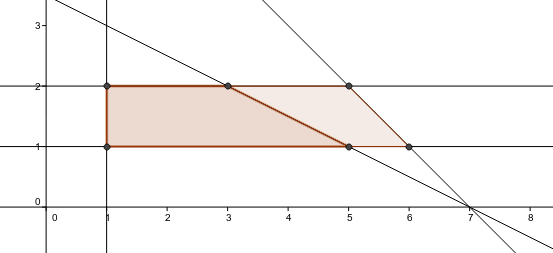
\includegraphics[width=0.5\textwidth]{figs/cspace_example.png}
	\caption{C-space of an asynchronous system and its corresponding synchronous system}
	\label{fig:cspaceComp}
\end{center}
\end{figure}

\section{Conclusion}

% \nocite{*}
\bibliographystyle{latex8}
\bibliography{dit-paper}

\end{document}
